\chapter{Bullet Physics}

Bullet Physics é uma biblioteca livre para uso comercial escrita na linguagem de programação C++. É capaz de detectar e resolver a colisão entre objetos, interações entre articulações, além de simulações de tecidos e fluídos (BULLET, 2015).

A biblioteca é estruturada para ser utilizada como um todo ou apenas em parte. Pode-se utilizar somente a função de detecção de colisão, apenas o componente de \textit{rigid body} ou \textit{soft body} separadamente, ou mesmo somente a biblioteca de cálculos.

\begin{figure}[H]
	\centering
	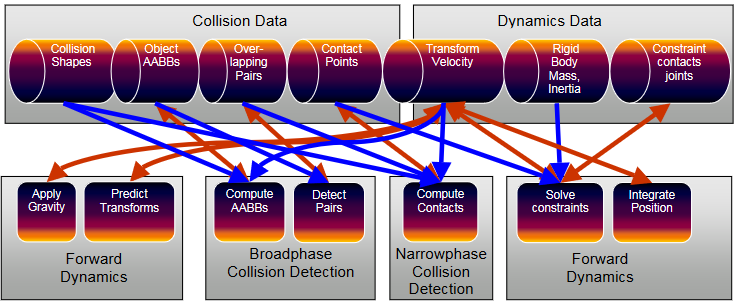
\includegraphics[scale=0.7]{imagens/bullet-pipeline.png}
	\caption{\small \textit{Pipeline} Bullet Physics (Fonte: BULLET, 2015)}
	\label{fig:bulletpipeline}
\end{figure}

A figura \ref{fig:bulletpipeline} apresenta os passos executados na implementação padrão, chamada de \lstinline{btDiscreteDynamicsWorld}. Assim como no objeto que engloba o modelo físico aplicado, outros objetos também possuem o prefixo \lstinline{bt}, como o \lstinline{btScalar}, que representa um número de ponto flutuante e \lstinline{btVector3}, um vetor de 3 posições. Tais abstrações são importantes porque fornecem métodos úteis para a biblioteca encapsulados, além de manter compatibilidade entre diferentes sistemas, uma vez que podemos utilizar  \lstinline{btscalar} independente da implementação do sistema.

